% App. F (new, 2026-11-12): the earlier evaluation run behind the gait
% statistics (fig:gait, fig:swing-transfer a) and the frames (fig:frames). Not
% the runs of Table 1.
% 2026-11-13 (author's new focus): the fig:frames float moved here from the
% Results (no main-text reference to it remains), and the definitions behind
% the acyclicity measures added ("Period and stepping order"; macros
% \corlGaitEventRepeatPct ff. in constants.tex, reproduced from timming.md by
% the session script writerB/acyclicity_stats.py, counts below from its output).
% 2026-11-13 appendix pass (author: "only the math needed ... add the
% important things"): kept the disclosure of the run, the swing detector, the
% overlap counts, the definitions of the measures used in Sec. 5 and the
% frames. Cut:
% this run's six per-cell success rates (CADENCE 100/93/96 and 96/87/77, trot
% 97/89/80 and 94/81/63 of 100, at 0.10 and 0.20 m/s), the step rates
% (\corlGaitStepsSlow / \corlGaitStepsFast steps/s against the trot's
% \corlGaitStepsTrot), the growth of non-diagonal pairs with difficulty
% (\corlGaitNonDiagEasy to \corlGaitNonDiagHard per trial), the "no share of
% time with all feet down" remark, the step cap of CADENCE-Single (it used the
% sweep's unconfirmed steps per metre, \corlOcsStepsPerM*, and is cited
% nowhere), and the video file names in the prose (now in the comment above
% the frames paragraph).
% Sources: rss/timming.md (CSV, one row per measured swing; author,
% 2026-11-04) analysed by figures/gait_stats.py (report re-run on 2026-11-12:
% pairs 24370 diagonal / 227 rear / 158 side / 38 front = 24793; diagonal
% lift-off lag median 42 ms, q10-q90 21-66 ms; trot same sample 96.9 %;
% measured swing medians 0.128 s / 0.235 s over 55170 / 53431 field swings;
% 23.8 % of CADENCE's field swings below 0.1 s; the CV is std/mean of the
% same-leg lift-off intervals pooled over legs, cells and successful trials).
% Rules (rewrite_decisions.md): do not name this run's training seed or
% iteration; it is on other worlds than Table 1 (author); no success rate in
% the main text comes from it.
% AUTHOR TODO: state what else changed between this run and the Table 1 runs
% (how the worlds are built, depth pipeline, Gazebo/OCS2 version, criterion); the trot
% fell from 84.0 % here to 67.8 % in Table 1.
% The swing detector's threshold (1.5 cm above a rolling minimum) is only
% presumed in gait_stats.py, so no value is printed.

\section{Earlier Evaluation Run: Gait Statistics and Frames}
\label{app:earlier-run}

\noindent\textbf{The run.}
\looseness=-1 The gait statistics of Figs.~\ref{fig:gait}
and~\ref{fig:swing-transfer}a and the frames of Fig.~\ref{fig:frames}b
come from an earlier evaluation run on OCS2, not from the runs of
Table~\ref{tab:results}. It ran one CADENCE policy, deployed as in
Sec.~\ref{subsec:method-deployment} with an OCS2 IFM and depth-camera
terrain, and OCS2's own trot. Its worlds differ from those of
Table~\ref{tab:results}, but it used the benchmark's six cells,
\corlBenchTrialsPerCell{} trials of \corlBenchTrialSeconds\,s per cell,
and the benchmark's success criterion. CADENCE succeeded in
\corlGaitTrialsGaitNet{} of \corlBenchTrialsPerArm{} trials (91.5\%) and
the trot in \corlGaitTrialsTrot{} (84.0\%). Both succeeded more often
than in Table~\ref{tab:results}, the trot by far more (84.0 against
\corlBenchTrot\%), so CADENCE's lead over the trot was 7.5 points in
this run against 17.3 in Table~\ref{tab:results}. No success rate in the
main text comes from this run, which we use only for the gait statistics
and the frames of Fig.~\ref{fig:frames}b. Fig.~\ref{fig:frames}a shows a
separate OCS2 trial of the same policy on a ramp track outside the
benchmark.

\noindent\textbf{Swing detection.}
\looseness=-1 The run's log holds one row per swing, taken from the
simulator's ground-truth foot heights: \verify{a foot counts as in swing
while its height is above a threshold}. The heights are sampled about
every 21\,ms of simulated time (median spacing, 20 to 34\,ms within a
trial), so each lift-off and touchdown is known to about one sample.
The statistics use only the successful trials, \corlGaitTrialsGaitNet{}
of CADENCE and \corlGaitTrialsTrot{} of the trot, and only the swings
that land on the \emph{void field}, between the time the rear feet reach
the voids and the end of the trial: \corlGaitSwingsGaitNet{} swings of
CADENCE and \corlGaitSwingsTrot{} of the trot. Since the trot failed
more often in the hardest cells, fewer of its trials there enter the
statistics, so the two methods are measured on different mixes of
trials. The detector also shortens swings. The trot, scheduled with
\corlTrotSwing\,s swings on a \corlTrotPeriod\,s period, measures a
median swing of \corlGaitTrotSwingMeasured\,s, although its median time
between a leg's lift-offs, \corlGaitTrotPeriodMeasured\,s, matches the
period. About a quarter of CADENCE's measured swings, moreover, fall
below its shortest commanded swing time of \corlSwingDurationMin\,s.
Hence the measured swing medians, \corlGaitSwingMedian{} and
\corlGaitSwingMedianTrot\,s, compare CADENCE with the trot under the
same detector and do not measure how long a swing lasted.

\noindent\textbf{Overlapping swings.}
\looseness=-1 Two swings of different legs overlap when their measured
intervals intersect. Of CADENCE's \corlGaitOverlapPairs{} overlapping
pairs, 24{,}370 (\corlGaitDiagPairPct\%) paired diagonal legs, 227 the
rear legs, 158 the two legs of one side, and 38 the front legs, whereas
all of the trot's pairs were diagonal. CADENCE's diagonal partners
lifted off a median \corlGaitLiftLagMs\,ms apart (10th to 90th
percentile, 21 to \corlGaitEventWindowMs\,ms). This is about one
\corlControlTickMs\,ms tick, the shortest gap that starting at most one
step per tick allows, measured to one or two samples. The trot's partners
lifted off in the same sample in 97\% of its pairs.

% Counts: writerB/acyclicity_stats.py on timming.md (2026-11-13), see the
% comment at \corlGaitEventRepeatPct in constants.tex.
\noindent\textbf{Period and stepping order.}
\looseness=-1 We call CADENCE's gait acyclic because neither its period
nor its stepping order is fixed, and we measure the two separately, on
the counted swings of each successful trial. A leg's time between
lift-offs runs from one of its lift-offs to its next. The coefficient
of variation (CV) of Fig.~\ref{fig:gait}b is the standard deviation of
these times over their mean, pooled over all legs, cells, and
successful trials, and it is \corlGaitStrideCv{} for CADENCE against
\corlGaitStrideCvTrot{} for the trot. A step rate is the number of
counted lift-offs on the void field per second of void-field time,
pooled over successful trials: \corlGaitStepsSlow{} and
\corlGaitStepsFast{} for CADENCE at \corlBenchSpeedSlow{} and
\corlBenchSpeedFast\,m/s, and \corlGaitStepsTrot{} for the trot. The stepping order is read from
each trial's sequence of lift-offs, sorted by lift-off time and, for
lift-offs in the same sample, by leg. A \emph{step event} groups the
lift-offs within \corlGaitEventWindowMs\,ms of its first one. This
window is the 90th percentile of the lift-off lag between CADENCE's
diagonal partners, so an event holds the legs that lift together, and
grouping instead by gaps of at most \corlGaitEventWindowMs\,ms between
successive lift-offs gives the same result. The first measure is how
often a step event lifts the same set of legs as the one before it,
the second how often a leg lifts \emph{twice in a row}, that is, two
consecutive lift-offs are of the same leg, and the third how often four
consecutive lift-offs cover all four legs. \verify{The first held for
5{,}102 of CADENCE's 32{,}186 pairs of consecutive events
(\corlGaitEventRepeatPct\%) and for none of the trot's 26{,}214, the
second for 3{,}338 of CADENCE's 54{,}621 pairs of consecutive lift-offs
(\corlGaitLegTwicePct\%) and for none of the trot's 52{,}927, and the
third for 21{,}565 of CADENCE's 53{,}523 overlapping windows of four
(\corlGaitFourAllPct\%) and for 51{,}561 of the trot's 51{,}919
(\corlGaitFourAllPctTrot\%).} A commanded swing lasts at least
\corlSwingDurationMin\,s, longer than the event window, so under the
contact rule an event of commanded steps holds at most
\numberstringnum{\corlMaxConcurrentSwingLegs} legs. A gait that lifts
each leg once per cycle in a fixed order therefore has at least two
events per cycle and scores 0, 0, and 100\% on these three measures.
Like the other statistics, these are measured on successful trials only
and to about one sample.

\begin{figure}[t]
  \centering
  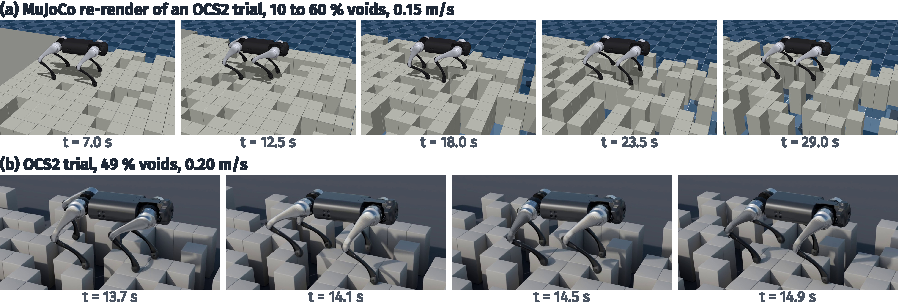
\includegraphics[width=\textwidth]{figures/fig_frames}
  \caption{CADENCE on OCS2, not the runs of Table~\ref{tab:results}.
    (a)~A separate OCS2 trial on a track whose voids
    ramp from 10 to 60\%, at 0.15\,m/s, re-rendered in MuJoCo; with no
    state log, the void fraction under the robot is not known. (b)~An
    OCS2 trial of the earlier evaluation run, at \corlBenchVoidHigh\% voids
    and \corlBenchSpeedFast\,m/s.}
  \label{fig:frames}
\end{figure}

\noindent\textbf{Frames.}
\looseness=-1 Fig.~\ref{fig:frames} shows two OCS2 trials of this run's
CADENCE policy: (a)~on a track whose voids ramp from 10 to 60\% at
0.15\,m/s, re-rendered in MuJoCo, and (b)~at \corlBenchVoidHigh\% voids
and \corlBenchSpeedFast\,m/s. They illustrate the stepping only; no
claim rests on them.
